\documentclass{paper}

%\usepackage{times}
\usepackage{epsfig}
\usepackage{graphicx}
\usepackage{amsmath}
\usepackage{amssymb}
\usepackage{color}
\usepackage{mathtools}




\usepackage{caption}
\usepackage{float}
\usepackage{subfigure}


% load package with ``framed'' and ``numbered'' option.
%\usepackage[framed,numbered,autolinebreaks,useliterate]{mcode}

% something NOT relevant to the usage of the package.
\setlength{\parindent}{0pt}
\setlength{\parskip}{18pt}






\usepackage[latin1]{inputenc} 
\usepackage[T1]{fontenc} 

\usepackage{listings} 
\lstset{% 
   language=Matlab, 
   basicstyle=\small\ttfamily, 
} 

\newcommand{\norm}[1]{\left\lVert#1\right\rVert}
\DeclareMathOperator*{\argmin}{arg\,min}

\title{Assignment 1}



\author{Single Michael\\08-917-445}
% //////////////////////////////////////////////////


\begin{document}



\maketitle


% Add figures:
%\begin{figure}[t]
%%\begin{center}
%\quad\quad   \includegraphics[width=1\linewidth]{ass2}
%%\end{center}
%
%\label{fig:performance}
%\end{figure}

\section{Demosaicing}
In this work we will develop solution for the demosaicing problem when dealing with raw camera images. For that purpose we will formulate a convex optimization problem that is modeling the process of demosaicing a mosaiced image. We approximate our convex cost function by relying on the gradient descent and discretizing it using a forward difference scheme. We also examine the impact of the regularization parameter in our convex cost function by adjusting its value. Last, we describe how we can retrieve an optimal regularization term relying on SSD. 

\subsection{Motivation}
Most digital cameras acquire images from an image sensor overlaid with a color filter array (CFA). A color filter array depicts a mosaic of RGB color filters applied in front of the image sensor. An example is illustrated in figure $FIGURE$. This implies that each pixel in a raw camera image stores only the measured color channel value that corresponds to its pixel-position in the CFA. In other words, each pixel in a raw camera image represents one RGB color. Its color value depends on the color filter that is applied to that pixel. 

Such a raw filter image does no look like we humans are used to see images. Therefore goal is to reconstruct the missing color channel information from the pixel's neighborhood. The described problem is also known as \emph{demosaicing}. One particular way how to address this problem is by is by billinearly interpolating the missing color information from a pixel's neighborhood. This is straight forward approach and can be implemented by solving a huge sparse linear system of equations. However, the resulting image may exhibits notable artifacts - colorfull fringes along texture-boundaries. Usually, this can be fixed by applying a non-linear filtering approach, such as a median filter. Such a filtering approach, however, assumes spatial coherence of the raw image's pixel.

Since this approach is less mathematical sound we focus on another approach in this project. We try to formulate the the demosaicing task as a convex minimization problem.     

\subsection{Problem Statement}
In this work we address the problem of demosaicing by formulating it as a convex optimization problem. Given a mosaiced image $g$ depicting a raw camera production, we want to find an optimal demosaiced image $u$. For describing the optimality property we take into account a cost function that describes the color smoothness and also that the resulting image $u$ should be close to the given raw input image $g$. 

More precisely, let $g$ denote the bayer filter camera raw input image. Then we want to solve for $u=(u_r, u_g, u_g)$ (RGB image) minimzating the following energy term (cost function):

\begin{align}
	E(u_c) = \norm{\nabla u_c}_2 + \frac{\lambda}{2} \norm{u_c - g}^2_{\Omega_{c}}
\label{eq:basis_cost_demosaicing}	
\end{align}

with the measure

\begin{equation}
	\norm{u_C - g}^2_{\Omega_{C}} = \sum_x \sum_y \Omega_{C}(x,y)\norm{u_{c}(x,y) - g(x,y)}^2
\label{eq:measure}
\end{equation}

where C denotes the three different color channels. $\Omega_{C}$ is defined such that $\Omega_{C}(x,y) = 1$ if the pixel value at $(x,y)$ is \emph{valid}$\footnote{this means that the pixel at location (x,y) is valid for the bayer color mask C}$ and $\Omega_{C}(x,y) = 0$ when the data is missing.

The cost function from equation $\ref{eq:basis_cost_demosaicing}$ consists of a smoothness term, $\norm{\nabla u_c}_2$ and $\norm{u_c - g}^{2}_{\Omega_{c}}$. The first term ensures a smooth color transition between colors in a l2 norm sense. The second term ensures that the reconstructed images does not deviate too much from the given input, i.e. de demosaiced image should resemble to the provided mosaiced raw camera image. This similarity term is further parameterized by a regularization term $\lambda$, indicating how strong the output should match the given input according to the formulated measure in equation $\ref{eq:measure}$. In summary, larger values for $\lambda$ weight the similarity of the input and output image more, and contrarely, lower values weight the color smoothness term more.

Hereby, minimizating the cost function from equation $\ref{eq:basis_cost_demosaicing}$ leads to an optimal demosaiced image $u$.
Mathematically we want to solve for 

\begin{equation}
	\widetilde{u} = \argmin_{u_c} E(u_c)
\label{eq:our_general_cost_function}
\end{equation}

We can further simplify the cost function stated in equation $\ref{eq:basis_cost_demosaicing}$ relying on the following observation: Since the function $\Omega_{C}$ is only true for pixels that correspond to the color channel C in the bayer mask, we see that $\Omega_{C}(x,y)\norm{u_{c}(x,y) - g(x,y)}$ is only not equal zero if the pixel at location $(x,y)$ belongs to the color channel $C$. Therefore we are allowed to solve the stated optimization problem from equation $\ref{eq:basis_cost_demosaicing}$ for each color channel separately. 


According to this insight we are supposed to minimize the following three independent$\footnote{Independent in the sense that we are allowed to solve for each color channel separately}$ convex problems:

\begin{align}
	\widetilde{u_R} = \argmin_{u_R} \norm{\nabla u_R}_2 + \frac{\lambda}{2} \norm{u_R - g}^2_{\Omega_{R}} \nonumber \\
	\widetilde{u_G} = \argmin_{u_G} \norm{\nabla u_G}_2 + \frac{\lambda}{2} \norm{u_G - g}^2_{\Omega_{G}}\nonumber \\
	\widetilde{u_B} = \argmin_{u_B} \norm{\nabla u_R}_2 + \frac{\lambda}{2} \norm{u_B - g}^2_{\Omega_{B}}
\label{eq:our_convex_probelm}		
\end{align}

Where we still rely on the measure defined in equation $\ref{eq:measure}$ but C was replayed by the appropriate color channel$\footnote{C stands for either the color channel R, G or B.}$. We notice that the equations in $\ref{eq:our_convex_probelm}$ tell us that we have to solve three different energies similar to the one formulated in equation $\ref{eq:our_general_cost_function}$.

In the next section we will describe how to solve the stated minimization problems from equation $\ref{eq:our_convex_probelm}$ numerically.

\subsection{Methodology}

In the previous section we have formulated the demosaicing task as a convex optimization problem shown in equation $\ref{eq:our_convex_probelm}$. In this section we describe the method we will use for computing the solution of our stated minimization problem.

To minimize our cost function $E$ as required in equation $\ref{eq:our_general_cost_function}$, we rely on the \emph{gradient descent} approach. This is an iterative method that can be used to solve energy minimiazion problems, such as our cost function. In detail, the following steps have to be performed when implementing the gradient descent approach:
\begin{enumerate}
	\item Choose a random initial point $x_0$ for starting the iteration. 
	\item Apply the following update rule:
		\begin{align}
			x_{n+1} = x_n - \alpha \nabla{E(x_n)} 
		\end{align}
	\item Iterate until the update rule converges, i.e. $\norm{x_{n+1}-x_n} \leq \epsilon$
\end{enumerate} 

The variable $x_n$ depicts the unknown variable at iteration step $n$ we are looking for. $E(x_n)$ is the cost function that we aim to minimize, the parameter $\alpha$ describes the learning rate of the gradient descent method. It is responsible for the convergence rate of the method. If is is chosen too large, the method will eventually diverge, if chosen too small it will require too many iterations. If the distance $\footnote{w.r.t some given norm}$ between the current and the previous iteration is below a given threshold $\epsilon$ we have found a satisfying iterative solution for our unknown variable $x$, that is $x_{n+1}$.

So, applying this method to our problem, $x$ corresponds to the unknown demosaiced image $u$ and $E$ is the cost function from equation $\ref{eq:our_general_cost_function}$. Therefore, for the color channel $c$$\footnote{c denotes the substitute for either one of the following r,g,b color channels.}$ the gradient descend formulation of our problem is defined as the following:

\begin{align}
	u_{c}^{n+1}(i,j) = u_{c}^{n}(i,j) - \alpha \frac{\partial{E}}{\partial{u^{n}_{c} (i,j)}}(i,j)
\label{eq:our_gradient_descend_method}	
\end{align}

Equation $\ref{eq:our_gradient_descend_method}$ describes how we have to update a pixel at location (x,y) for the color channel $c$ using the gradient descend method. The index $n$ denotes the current iteration index. 

We see, that this method needs an identity for the partial derivative applied on our cost function. In the following use omit the iteration index $n$ for the iterative solution $u_{c}^{n+1}$ from equation $\ref{eq:our_gradient_descend_method}$ and instead use the abbriviation $u_{c}$.

Since the data we are dealing with (pixels) is in a discrete domain, we have to discretize the expression $\frac{\partial{E}}{\partial{u_{c} (i,j)}}$. The discretization of this expression is described in the next section.  

\subsection{Derivations}

In this subsection we derive an explicit approximation for the the partial derivative of our energy term $E$ that can be numerically computed. Such an approximation is useful since we will need its expression later for our update rule to solve our demosaicing optimization problem. For the discretization we will relying on a forward difference scheme. By the end of this section we will have derived an discretization of the expression $\frac{\partial{E}}{\partial{u_{c} (i,j)}}(i,j)$.

We start our derivation by simplifying the definition $\frac{\partial{E}}{\partial{u_{c} (i,j)}}(i,j)$.

\begin{align}
	\frac{\partial{E}}{\partial{u_{c} (i,j)}}(i,j)
	&= \frac{\partial}{\partial{u_{c} (i,j)}} \left( \norm{\nabla u_c}_2 + \frac{\lambda}{2} \norm{u_c - g}^2_{\Omega_{c}} \right) \nonumber \\
	&= \frac{\partial}{\partial{u_{c} (i,j)}} \left( \norm{\nabla u_c}_2 + \frac{\lambda}{2} \left( \sum_{i'=1}^M \sum_{j'=1}^N \Omega_{C}(i',j')\norm{u_{c}(i',j') - g(i',j')}^2
\right) \right) \nonumber \\
&= \frac{\partial}{\partial{u_{c} (i,j)}} \norm{\nabla u_c}_2 + \frac{\lambda}{2} \frac{\partial}{\partial{u_{c} (i,j)}}  \left( \sum_{i'=1}^M \sum_{j'=1}^N \Omega_{C}(i',j')\norm{u_{c}(i',j') - g(i',j')}^2
\right) \nonumber \\
&= \frac{\partial}{\partial{u_{c} (i,j)}} \norm{\nabla u_c}_2 + \frac{\lambda}{2} \left( \sum_{i'=1}^M \sum_{j'=1}^N \frac{\partial}{\partial{u_{c} (i,j)}} \Omega_{C}(i',j')\norm{u_{c}(i',j') - g(i',j')}^2
\right) \nonumber \\
&= \frac{\partial}{\partial{u_{c} (i,j)}} \norm{\nabla u_c}_2 + \frac{\lambda}{2} \frac{\partial}{\partial{u_{c} (i,j)}} \left( \Omega_{C}(i,j)\norm{u_{c}(i,j) - g(i,j)}^2 \right) \nonumber \\
&= \frac{\partial}{\partial{u_{c} (i,j)}} \norm{\nabla u_c}_2 + \frac{\lambda}{2} 2 \Omega_{C}(i,j) \left( u_{c}(i,j) - g(i,j) \right) (1-0) \nonumber \\
&= \frac{\partial}{\partial{u_{c} (i,j)}} \norm{\nabla u_c}_2 + \lambda \Omega_{C}(i,j) \left( u_{c}(i,j) - g(i,j) \right)
\label{eq:part_deriv_e}
\end{align}

The key step for the derivation of equation $\ref{eq:part_deriv_e}$ is based on the following observation: 

$$ \forall (i',j')  \neq (i,j): \frac{\partial}{\partial{u_{c} (i,j)}} \Omega_{C}(i',j')\norm{u_{c}(i',j') - g(i',j')}^2 = 0 $$
Which states that every index pair $(i',j')$ not equal to $(i,j)$ has a zero derivative along the direction $u_c(i,j)$. Another important fact we used for the derivation was that 

\begin{align}
	\Omega_{c}(i',j')\norm{u_{c}(i',j') - g(i',j')}^2
	&= \sum_{c'\in \{ r,g,b \}} \Omega_{c'}(i',j')\norm{u_{c'}(i',j') - g(i',j')}^2 \nonumber \\
	&= \Omega_{c'}(i',j')\left( u_{c'}(i',j') - g(i',j') \right)
\end{align}

For the current valid color channel $c'$. In other words, all other color channel components of the rgb vector have a zero value contribution except the currently selected channel $c'$.

Next we have to derive an expression for the partial derivative applied in the two norm, i.e. $\frac{\partial}{\partial{u_{c} (i,j)}} \norm{\nabla u_c}_2$. For this purpose we make use of a forward difference approximation scheme for the derivatives $\partial_{i} u_c$ and $\partial_{j} u_c$ respectively, we can derive the following expression for the regularization term:

\begin{align}
	 \norm{\nabla{u_{c}}}_2 
	&= \sum_{i=1}^N \sum_{j=1}^M \sqrt{[\partial_{i} u_c(i,j)]^2 + [\partial_{j} u_c(i,j)]^2} \nonumber \\ 
	&= \sum_{i=1}^N \sum_{j=1}^M \sqrt{\left[ u_{c}\left(i+1, j\right) - u_{c}\left(i,j\right) \right]^2 + \left[ u_{c}\left(i, j+1 \right) - u_{c}\left(i,j\right) \right]^2}
\label{eq:regularization_expr}
\end{align}

In oder to simplify later derivation steps, let us introduce the helper function $\tau$ defined as the following 

\begin{equation}
	 \tau_{c}\left(i,j\right)
	= \sqrt{\left[ u_{c}\left(i+1, j\right) - u_{c}\left(i,j\right) \right]^2 + \left[ u_{c}\left(i, j+1 \right) - u_{c}\left(i,j\right) \right]^2}
\label{eq:tau_function}	
\end{equation}

We notice that $\tau$ is only the expression under the summation in the right hand side in equation $\ref{eq:regularization_expr}$. Next, let us take the partial derivative along $u_{c}(i,j)$ of $\norm{\nabla{u_{c}}}_2$. By fixing a index pair ($i$ $j$) and reordering the terms under the summation, we see that 

\begin{equation}
	\frac{\partial}{\partial u_{c}\left(i,j\right)} \norm{\nabla{u_c}}_2 = \underbrace{\frac{\partial{\tau_{c}\left(i,j\right)}}{\partial u_{c}\left(i,j\right)}}_{\bf{(a)}} + \underbrace{\frac{\partial{\tau_{c}\left(i-1,j\right)}}{\partial u_{c}\left(i,j\right)}}_{\bf{(b)}} + \underbrace{\frac{\partial{\tau_{c}\left(i,j-1\right)}}{\partial u_{c}\left(i,j\right)}}_{\bf{(c)}}
\label{eq:abc_term}
\end{equation}

Next I will derive explicit expressions for the terms $\bf{(a)}$, $\bf{(b)}$ and $\bf{(c)}$. Loosely speaking our goal is to get rid of the partial derivative operator. The mathematical key concept I will rely on is the chain rule for partial derivatives. More precisely we will make use of the fact that $\partial_{x}\sqrt{f(x)}$ is $\frac{\partial_{x} f(x)}{2 \sqrt{f(x)}}$.

\begin{align}
	(a) \Longrightarrow
	& \frac{\partial{\tau_{c}\left(i,j\right)}}{\partial u_{c}\left(i,j\right)} \nonumber \\
	&= \frac{\partial}{\partial{u_{c}\left(i,j\right)}} \sqrt{ \left[u_{c}(i+1,j) - u_{c}(i,j)\right]^2 + \left[u_{c}(i,j+1) - u_{c}(i,j)\right]^2} \nonumber \\
	&= \frac{1}{2} \frac{2 (u_{c}(i+1,j)-u_{c}(i,j))(0-1) + 2 (u_{c}(i,j+1)-u_{c}(i,j))(0-1)}{\sqrt{ \left[u_{c}(i+1,j) - u_{c}(i,j)\right]^2 + \left[u_{c}(i,j+1) - u_{c}(i,j)\right]^2}} \nonumber \\
	&= \frac{1}{2} \frac{2 [-(u_{c}(i+1,j)-u_{c}(i,j)) - (u_{c}(i,j+1)-u_{c}(i,j)]}{\tau_{c}\left(i,j\right)} \nonumber \\
	&= \frac{2 u_{c} \left(i,j\right) - u_{c} \left(i+1,j\right)-u_{c} \left(i,j+1\right)}{\tau_{c}\left(i,j\right)}
\label{eq:a_term}	
\end{align}

\begin{align}
(b) \Longrightarrow
	& \frac{\partial{\tau_{c}\left(i-1,j\right)}}{\partial u_{c}\left(i,j\right)} \nonumber \\
	&= \frac{\partial}{\partial{u_{c}\left(i,j\right)}} \sqrt{ \left[u_{c}(i,j) - u_{c}(i-1,j)\right]^2 + \left[u_{c}(i-1,j+1) - u_{c}(i-1,j)\right]^2} \nonumber \\
	&= \frac{1}{2} \frac{2[\left(u_{c}(i,j) - u_{c}(i-1,j)\right)(1-0) + \left(u_{c}(i-1,j+1) - u_{c}(i-1,j)\right)(0-0)]}{\sqrt{ \left[u_{c}(i,j) - u_{c}(i-1,j)\right]^2 + \left[u_{c}(i-1,j+1) - u_{c}(i-1,j)\right]^2}} \nonumber \\
	&= \frac{1}{2} \frac{2\left[(u_{c}(i,j) - u_{c}(i-1,j)\right]}{\tau_{c}\left(i-1,j\right)} \nonumber \\
	&= \frac{u_{c}\left(i,j\right) - u_{c}\left(i-1,j\right)}{\tau_{c}\left(i-1,j\right)}
\label{eq:b_term}	
\end{align}

\begin{align}
(c) \Longrightarrow
	& \frac{\partial{\tau_{c}\left(i,j-1\right)}}{\partial u_{c}\left(i,j\right)} \nonumber \\
	&= \frac{\partial}{\partial{u_{c}\left(i,j\right)}} \sqrt{ \left[u_{c}(i+1,j-1)-u_{c}(i,j-1)\right]^2 + \left[u_{c}(i,j) - u_{c}(i,j-1)\right]^2} \nonumber \\
	&=  \frac{1}{2} \frac{2 [\left(u_{c}(i+1,j-1)-u_{c}(i,j-1)\right)(0 - 0) + \left(u_{c}(i,j) - u_{c}(i,j-1)\right)(1-0)]}{\sqrt{ \left[u_{c}(i+1,j-1)-u_{c}(i,j-1)\right]^2 + \left[u_{c}(i,j) - u_{c}(i,j-1)\right]^2}} \nonumber \\
	&= \frac{1}{2} \frac{2 \left[u_{c}(i,j)- u_{c} (i,j-1)\right] }{\tau_{c}\left(i,j-1\right)} \nonumber \\			
	&= \frac{u_{c}(i,j)-u_{c} \left(i,j-1\right)}{\tau_{c}\left(i,j-1\right)}
\label{eq:c_term}	
\end{align}

Using the findings from the equations $\ref{eq:a_term}$, $\ref{eq:b_term}$ and $\ref{eq:c_term}$ and plug them into into equation $\ref{eq:abc_term}$ we get its final numerical identity:

\begin{align}
\frac{\partial}{\partial u_{c}\left(i,j\right)} \norm{\nabla{u_c}}_2 
&= \Bigg(\frac{2 u_{c} \left(i,j\right) - u_{c} \left(i+1,j\right)-u_{c} \left(i,j+1\right)}{\tau_{c}\left(i,j\right)} \nonumber \\ 
&+ \frac{u_{c}\left(i,j\right) - u_{c}\left(i-1,j\right)}{\tau_{c}\left(i-1,j\right)} \nonumber \\
&+ \frac{u_{c}(i,j)-u_{c} \left(i,j-1\right)}{\tau_{c}\left(i,j-1\right)}\Bigg)
\label{eq:plugged_abc}	
\end{align}

In the next section we will present the final update rule according to our last findings and derivations. Furthermore we describe what issues we have to address when implementing a script that solves our convex problem.

\subsection{Implementation of Demosaicing}

In this section we explain how the convex demosaicing can be implemented using the gradient descend method. Since the problem is currently underconstrainted we also will have to choose some boundary condition. But first off, we formulate the final update gradient descend update rule by plugging the resulting equation $\ref{eq:plugged_abc}$ into equation $\ref{eq:part_deriv_e}$. Doing so we get the following final update rule:

\begin{align}
	u_{c} (i,j)
	&= u_{c}(i,j) - \alpha \frac{\partial{E(u_c)}}{\partial{u_{c} (i,j)}}(i,j) \nonumber \\
	&= u_{c}(i,j) - \alpha \left( \frac{\partial}{\partial{u_{c} (i,j)}} \norm{\nabla u_{c}(i,j)}_2 + \lambda \Omega_{C}(i,j) \left( u_{c}(i,j) - g(i,j) \right) \right) \nonumber \\
&\begin{aligned}
  =u_{c}(i,j) - \alpha \Bigg( \lambda \Omega_{C}(i,j) \left( u_{c}(i,j) - g(i,j) \right) &+ \frac{2 u_{c} \left(i,j\right) - u_{c} \left(i+1,j\right)-u_{c} \left(i,j+1\right)}{\tau_{c}\left(i,j\right)} \\
  &+ \frac{u_{c}\left(i,j\right) - u_{c}\left(i-1,j\right)}{\tau_{c}\left(i-1,j\right)} \\ 
  &+ \frac{u_{c}(i,j)-u_{c} \left(i,j-1\right)}{\tau_{c}\left(i,j-1\right)}\Bigg) \\
\end{aligned}
\label{eq:final_update_rule}
\end{align}

We only have to define a function that implements the final update rule from equation $\ref{eq:final_update_rule}$. This function is then evaluated for each given color channel. Assuming we have computed the approximations for all color channels, we only have to combine all intermediate results to an RGB image$\footnote{In Matlab this can be achieved by using the function reshape.}$.
Note that our update rule uses the auxiliary function $\tau$ defined as in equation $\ref{eq:tau_function}$. Note that $\tau(i,j)$ queries the indices $(i+1)$ and $(j+1)$. Furthermore, our update rule uses the indices (i+1) and (j+1) for some of its $u_c$ terms. Hence, when plugging the index (i+1) into $\tau$, for example, then the index $u(i+2,j)$ will be accessed. Similarly, some terms in our update rule access the index (i-1). When plugging this index into $\tau$ the query $u_c(i-2, j)$ will be performed. Analogues, for the indices j. 

This observation tells us, that we have to extend the images $g$ and $u$ by a 2 pixel width and height border. In other words, the images $u$, $g$ are extended by 2 pixels on the left, on the right, on top and on the bottom. This extension depicts our \emph{boundary condition} (BC). Defining a explicit BC will fully constraint our system and will finally allow us to solve the optimization problem. Note once chosen a particular BC and found an iterative solution, this introduced boundary can simply be truncated. This ensures the same dimensionality as we initially had.

For choosing the BC we have several possibilities. For my implementation I only experimented with the \emph{Dirichlet BC}, that directly constraint the pixel value of the boundary pixels. Another possibility would have been to try out von Neumann BC by constraing the derivatives on the boundary directly. However, I did not try this out, since as far as I understand my problem it is less related to some velocity vector field. The demosaicing is rather supposed to denote a spatial coherent problem. For such problems there is rather a constant velocity field present. This intuition made me choose the Dirichlet BC. 
There are different choices for defining Dirichlet BC. We could think of simply assigning the value zero on the boundary$\footnote{This corresponds to zero padding}$, define some axial symmetry$\footnote{This means that the boundary axis depicts the mirror axis. I.e. u(d, y) = u(-d,y)} and so forth.$ or assume that the image is periodically repeated. I tried all three variants and got the best results using a symmetric BC.
% TODO show some images when using different Dirichlet BCs

The update uses the learning rate parameter $\alpha$. I used a pretty small value for it of $\alpha=0.001$. Using this value for alpha resulted in convergence of my results. Note that I determined this value by a try and error approach. The only free parameter left to be retrieved is hence the regularization term $\lambda$.

In the next section I will demonstrate some results I get when using my demosaicing function for different $\lambda$ values. 

\subsection{Experimenting with different $\lambda$ values}

\begin{figure}[h!]
\begin{center}
  \subfigure[$\lambda=1$]{
   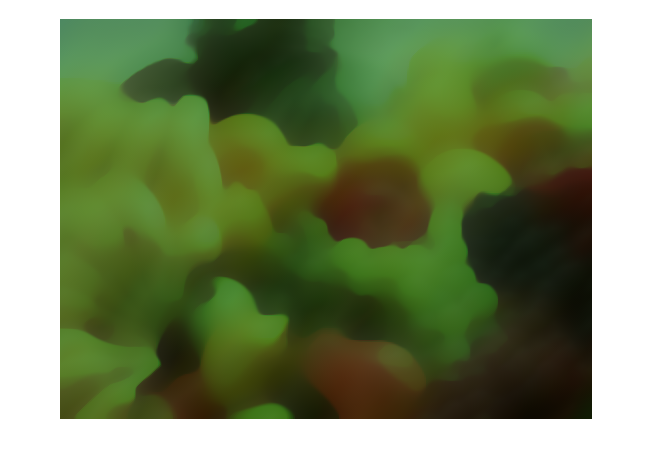
\includegraphics[scale =0.16] {figures/fruits_l1i1000Big}
   \label{fig:subfig1}
 }
 \subfigure[$\lambda=5$]{
   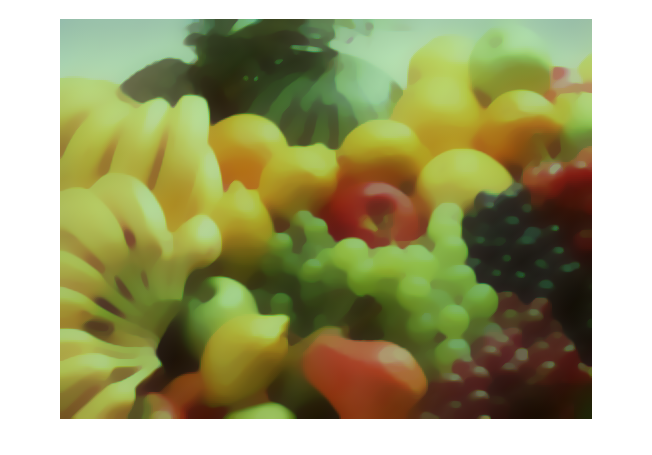
\includegraphics[scale =0.16] {figures/fruits_l5i1000Big}
   \label{fig:subfig2}
 }
 \subfigure[$\lambda=10$]{
   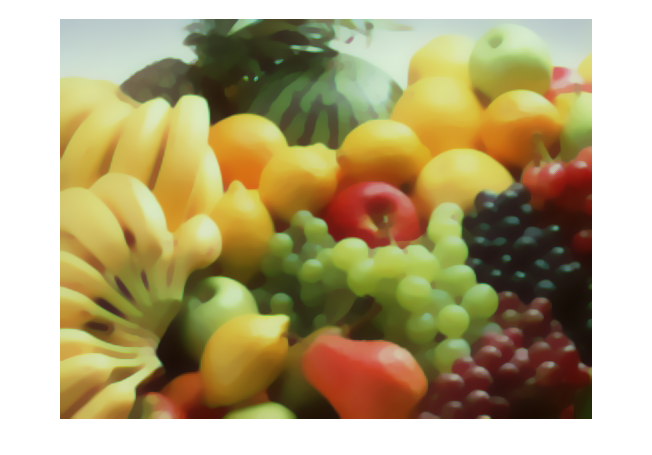
\includegraphics[scale =0.16] {figures/fruits_l10i1000Big}
   \label{fig:subfig3}
 }
 ~
  \subfigure[$\lambda=20$]{
   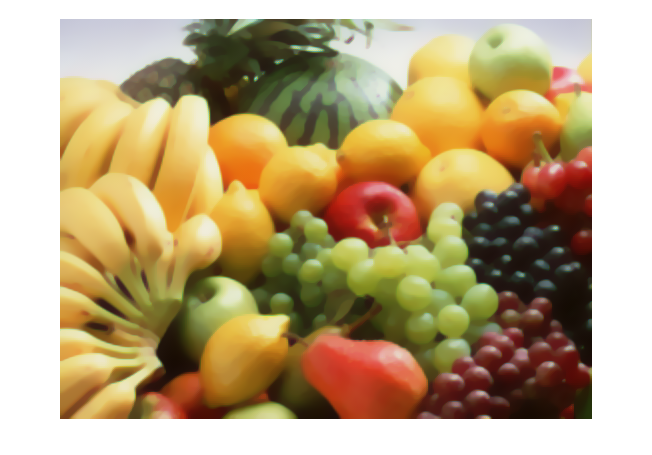
\includegraphics[scale =0.16] {figures/fruits_l20i1000Big}
   \label{fig:subfig4}
 }
 \subfigure[$\lambda=50$]{
   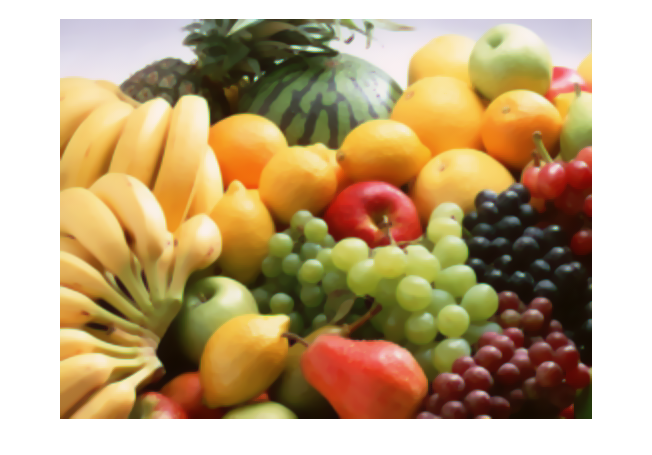
\includegraphics[scale =0.16] {figures/fruits_l50i1000Big}
   \label{fig:subfig5}
 }
 \subfigure[$\lambda=1950$]{
   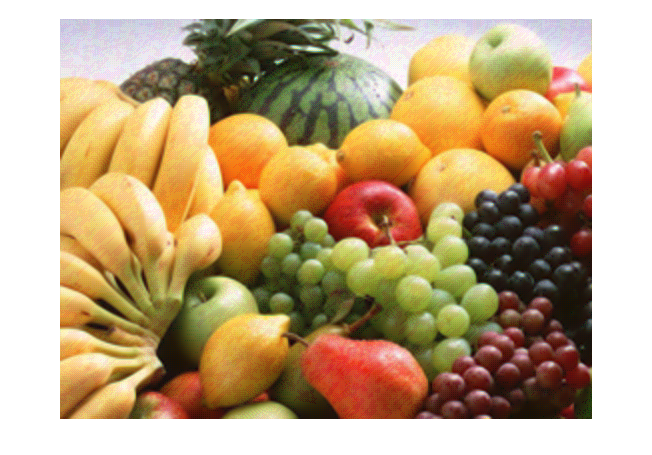
\includegraphics[scale =0.16] {figures/fruits_l1950i1000Big}
   \label{fig:subfig6}
 }
 ~
  \subfigure[$\lambda=2000$]{
   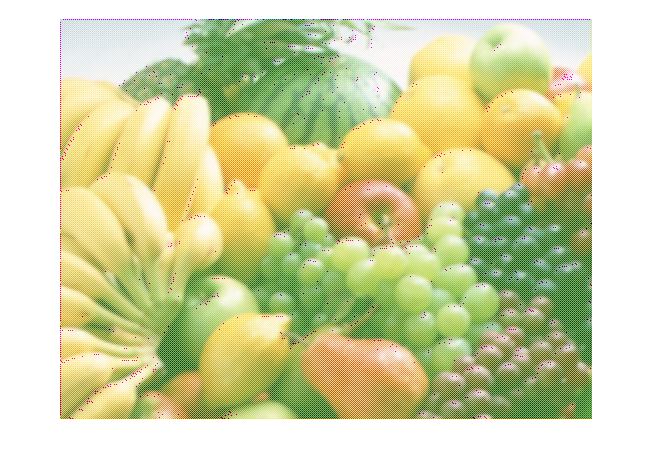
\includegraphics[scale =0.16] {figures/fruits_l2000i1000Big}
   \label{fig:subfig7}
 }
 \subfigure[$\lambda=2020$]{
   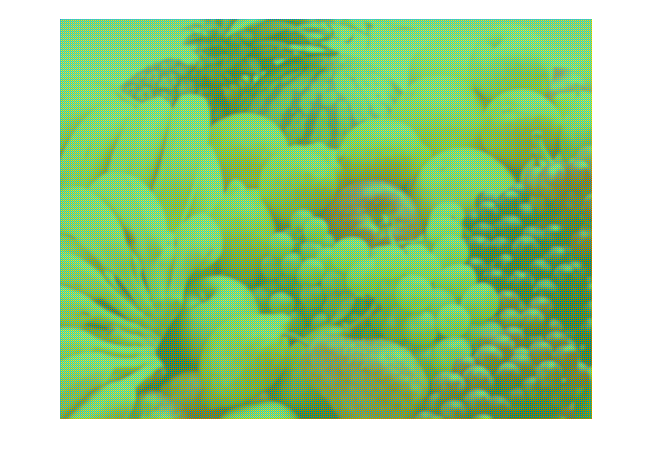
\includegraphics[scale =0.16] {figures/fruits_l2020i1000Big}
   \label{fig:subfig8}
 }
 \subfigure[$\lambda=2400$]{
   
\includegraphics[scale =0.16] {figures/fruits_l2400i1000Big}
   \label{fig:subfig9}
 }
\end{center}

\label{fig:many_different_lambda_values}
\caption{Reconstructed demosaicing results when using different values for $\lambda$ when running 1000 iterations.}
\end{figure}


\begin{figure}[h!]
\begin{center}
  \subfigure[$\lambda=1$]{
   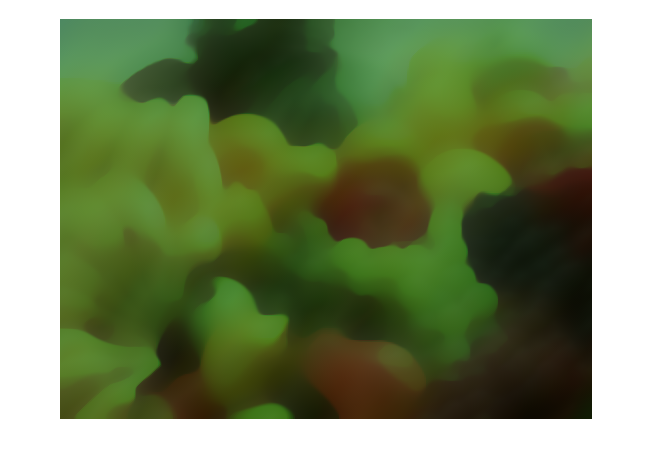
\includegraphics[scale =0.4] {figures/fruits_l1i1000Big}
   \label{fig:subfig11}
 }
~
 \subfigure[$\lambda=50$]{
   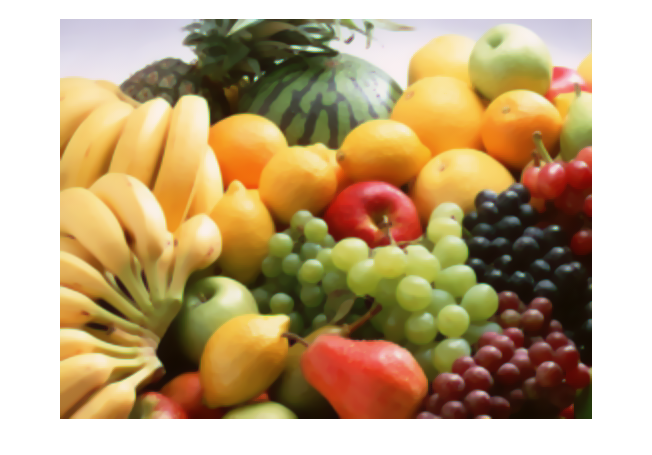
\includegraphics[scale =0.4] {figures/fruits_l50i1000Big}
   \label{fig:subfig12}
 }
 ~
  \subfigure[$\lambda=2000$]{
   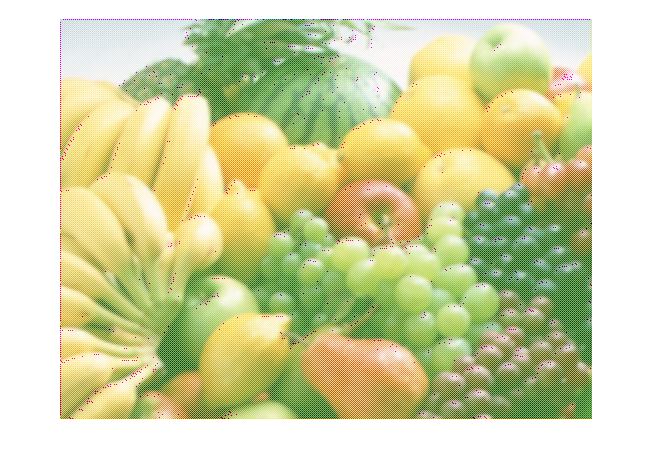
\includegraphics[scale =0.4] {figures/fruits_l2000i1000Big}
   \label{fig:subfig13}
 }

\end{center}

\label{fig:three_different_lambda_values}
\caption{Resized version of some good examples from figure $\ref{fig:many_different_lambda_values}$ illustrating the impact of the regularization parameter $\lambda$}
\end{figure}
 
 











\subsection{Optimal $\lambda$ value}

\begin{enumerate}
\item \textbf{Implement gradient descent for demosaicing.} In this section you should:

\begin{itemize}
\item Show some images, as the the gradient method progresses iteration by iteration. Display the initial and the final image and 3 more images in between.
\end{itemize}

\item \textbf{Show images obtained by very high, very low and optimal $\lambda$.} In this section you should:

\begin{itemize}
\item Display 3 images with different $\lambda$ (very low, very high and optimal).
\item Describe the effect of $\lambda$ on the solution.
\end{itemize}

\item \textbf{ Find optimal $\lambda$.} In this section you should:

\begin{itemize}
\item Display the $SSD$ vs. $\lambda$ graph.
\item Describe the effect of $\lambda$ with respect to the $SSD$ between the ground truth and the solution image.
\end{itemize}


\end{enumerate}


 \end{document}
 
 